\documentclass{article}\usepackage{amsmath,amssymb,amsthm,tikz,tkz-graph,color,chngpage,soul,hyperref,csquotes,graphicx,floatrow}\newcommand*{\QEDB}{\hfill\ensuremath{\square}}\newtheorem*{prop}{Proposition}\usepackage[shortlabels]{enumitem}\usepackage[nobreak=true]{mdframed}\usetikzlibrary{matrix,calc}\MakeOuterQuote{"}\usepackage[margin=1in]{geometry} \newtheorem{theorem}{Theorem} \usepackage{circuitikz}
\usepackage{tabto}
	\NumTabs{20}
\usepackage{fancyhdr}
\pagestyle{fancy}

\headheight=40pt
%New footer so your name gets on every page
%\rfoot{Your name here | Your SID here}

\renewcommand{\headrulewidth}{6pt}
\lhead{ \Large  \fontfamily{lmdh}\selectfont
CS 70	\tab Discrete Mathematics and Probability Theory
\\Spring 2017		\tab	\tab Satish Rao}
\rhead{\LARGE 	\fontfamily{lmdh}\selectfont	HW 0}

\begin{document}

\subsection*{1 Sundry}
\item Before you start your homework, write down your team. Who else did you work with on this homework? List names and email addresses. (In case of homework party, you can also just describe the group.) How did you work on this homework? Working in groups of 3-5 will earn credit for your "Sundry" grade.
\item Please copy the following statement and sign next to it:
\item \textit{I certify that all solutions are entirely in my words and that I have not looked at another student’s solutions. I have credited all external sources in this write up.}
\\
\\
Nadir Akhtar: nadir\_akhtar@berkeley.edu\\
Rustie Lin: rustielin@berkeley.edu\\
Raymond Feng: raymondhfeng@berkeley.edu\\
\\
    We primarily worked individually and checked our answers at the end but when someone got stuck we would try to figure out the issue as a group.\\

I certify that all solutions are entirely in my words and that I have not looked at another student’s solutions. I have credited all external sources in this write up. - Andy Zhang
\clearpage

%%%%%%%%%%%%%%%%%%%%%%%%%%%%%%%%%%%%%%%%%%%%%%%%%%%%%%%%%%%%%%%%%%%%%%%%%%

\subsection*{2 Problems}

\renewcommand{\labelenumii}{\Roman{enumii}}
\begin{enumerate}
\item \textbf{Lewis Caroll}

Here is an extract from Lewis Carroll's treatise \emph{Symbolic Logic} of 1896:
\begin{enumerate}
\item[(I)] No one, who is going to a party, ever fails to brush his or her hair.

\item[(II)] No one looks fascinating, if he or she is untidy.

\item[(III)] Opium-eaters have no self-command.

\item[(IV)] Everyone who has brushed his or her hair looks fascinating.

\item[(V)] No one wears kid gloves, unless he or she is going to a party.

\item[(VI)] A person is always untidy if he or she has no self-command.

\item[(a)] (3 points) Write each of the above six sentences as a quantified proposition over the universe of all people. You should use the following symbols for the various elementary propositions: $P(x)$ for ``$x$ goes to a party'', $B(x)$ for ``$x$ has brushed his or her hair'', $F(x)$ for ``$x$ looks fascinating'', $U(x)$ for ``$x$ is untidy'', $O(x)$ for ``$x$ is an opium-eater'', $N(x)$ for ``$x$ has no self-command'', and $K(x)$ for ``$x$ wears kid gloves''.
\begin{mdframed} \textbf{Solution} \\
\forall $x, P(x) \Rightarrow B(x)$\\
\forall $x, U(x) \Rightarrow \neg F(x)$\\
\forall $x, O(x) \Rightarrow N(x)$ \\
\forall $x, B(x) \Rightarrow F(x)$\\
\forall $x, K(x) \Rightarrow P(x)$ \\
\forall $x, N(x) \Rightarrow U(x)$ 
\end{mdframed}
\item[(b)] (2 points) Now rewrite each proposition equivalently using the contrapositive.
\begin{mdframed} \textbf{Solution} \\
\forall $x, \neg B(x) \Rightarrow \neg P(x)$\\
\forall $x, F(x) \Rightarrow \neg U(x)$\\
\forall $x, \neg N(x) \Rightarrow \neg O(x)$ \\
\forall $x, \neg F(x) \Rightarrow \neg B(x)$\\
\forall $x, \neg P(x) \Rightarrow \neg K(x)$ \\
\forall $x, \neg U(x) \Rightarrow \neg N(x)$ 
\end{mdframed}
\item[(c)] (2 points) You now have twelve propositions in total. What can you conclude from them about a person who wears kid gloves? Explain clearly the implications you used to arrive at your conclusion.
\begin{mdframed} \textbf{Solution} \\
A person who wears kid gloves is not an opium eater.\\
\\
People who wear kid gloves go to parties (a5). People who go to parties have brushed their hair (a1). People who have brushed their hair look fascinating (a4). People who look fascinating are not untidy (b2). People who are not untidy have self-command (b6). People who have self-command are not opium-eaters (b3). Thus, a person who wears kid gloves is not an opium-eater.
\end{mdframed}
\end{enumerate}

\item \textbf{Karnaugh Maps}

Below is the truth table for the boolean function

Y = (\lnot A \land \lnot B \land C) \lor (\lnot A \land B \land \lnot C) \lor (A \land \lnot B \land C) \lor (A \land B \land C).

%
\begin{center}
\begin{tabular}{ c | c | c || c }
$A$ & $B$ & $C$ & $Y$ \\
\hline
0 & 0 & 0 & 0 \\
0 & 0 & 1 & 1 \\
0 & 1 & 0 & 1 \\
0 & 1 & 1 & 0 \\
1 & 0 & 0 & 0 \\
1 & 0 & 1 & 1 \\
1 & 1 & 0 & 0 \\
1 & 1 & 1 & 1 
\end{tabular}
\end{center}

In this question, we will explore a different way of representing a truth table, the \emph{Karnaugh map}. A Karnaugh map is just a grid-like representation of a truth table, but as we will see, the mode of presentation can give more insight.  
The values inside the squares are copied from the output column of the truth table, so there is one square in the map for every row in the truth table. 

Around the edge of the Karnaugh map are the values of the input variables. Note that the sequence of numbers across the top of the map is not in binary sequence, which would be 00, 01, 10, 11. It is instead 00, 01, 11, 10, which is called \emph{Gray code} sequence. Gray code sequence only changes one binary bit as we go from one number to the next in the sequence. That means that adjacent cells will only vary by one bit, or Boolean variable.  In other words, \textit{cells sharing common Boolean variables are adjacent}.

For example, here is the Karnaugh map for $Y$:
%
\begin{figure}[htp]
\begin{center}
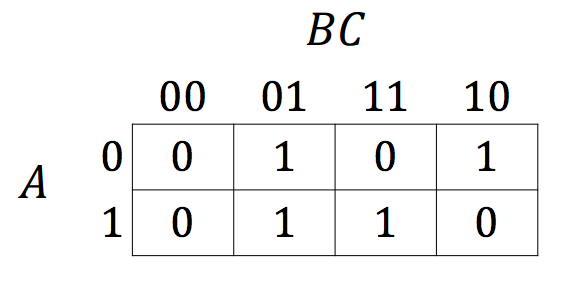
\includegraphics[width=4cm]{kmap1}
\end{center}
\end{figure}
%
The Karnaugh map provides a simple and straight-forward method of minimizing boolean expressions by visual inspection.  The technique is to examine the Karnaugh map for any groups of adjacent ones that occur, which can be combined to simplify the expression. Note that ``adjacent'' here means in the modular sense, so adjacency wraps around the top/bottom and left/right of the Karnaugh map; for example, the top-most cell of a column is adjacent to the bottom-most cell of the column.

For example, the ones in the second column in the Karnaugh map above can be combined because $(\lnot A \land \lnot B \land C)\lor (A \land \lnot B \land C)$ simplifies to $(\lnot B \land C)$. Applying this technique to the Karnaugh map (illustrated below), we obtain the following simplified expression for $Y$:
\begin{equation*}
Y = (\lnot B \land C) \lor (A \land C) \lor (\lnot A \land B \land \lnot C).
\end{equation*}
%
\begin{figure}[htp]
\begin{center}
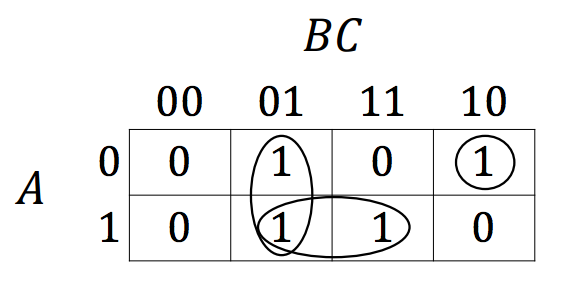
\includegraphics[width=4cm]{kmap2}
\end{center}
\end{figure}
%

\begin{enumerate}
\item[(a)] Write the truth table for the boolean function
\begin{align*}
    Z &= (\lnot A \land \lnot B \land \lnot C \land \lnot D) \lor (\lnot A \land \lnot B \land C \land \lnot D) \lor (A \land \lnot B \land \lnot C \land \lnot D) \\
      &\qquad \lor (A \land \lnot B \land C \land \lnot D).
\end{align*} 
\begin{mdframed} \textbf{Solution} \\
\begin{center}
\begin{tabular}{ c | c | c | c || c }
$A$ & $B$ & $C$ & $D$ & $Z$\\
\hline
0 & 0 & 0 & 0 & 1\\
0 & 0 & 0 & 1 & 0\\
0 & 0 & 1 & 1 & 0\\
0 & 0 & 1 & 0 & 1\\
0 & 1 & 0 & 0 & 0\\
0 & 1 & 0 & 1 & 0\\
0 & 1 & 1 & 1 & 0\\
0 & 1 & 1 & 0 & 0\\
1 & 1 & 0 & 0 & 0\\
1 & 1 & 0 & 1 & 0\\
1 & 1 & 1 & 1 & 0\\
1 & 1 & 1 & 0 & 0\\
1 & 0 & 0 & 0 & 1\\
1 & 0 & 0 & 1 & 0\\
1 & 0 & 1 & 1 & 0\\
1 & 0 & 1 & 0 & 1\\

\end{tabular}
\end{center}
\end{mdframed}


\item[(b)] Using your truth table, fill in the Karnaugh map for $Z$ below. \\

\begin{mdframed} \textbf{Solution} \\
\begin{center}
\begin{tabular}{llllll}
                     & \multicolumn{5}{c}{\textit{CD}}                                                                                                     \\
\multicolumn{1}{c}{} & & 00 & 01 & 11 & 10\\ 
\cline{3-6} 
\multicolumn{1}{c}{} & \multicolumn{1}{l|}{00} & \multicolumn{1}{l|}{\textcircled{1}} & \multicolumn{1}{l|}{0} & \multicolumn{1}{l|}{0} & \multicolumn{1}{l|}{\textcircled{1}} \\ 
\cline{3-6} \textit{AB} & 
\multicolumn{1}{l|}{01} & \multicolumn{1}{l|}{0} & \multicolumn{1}{l|}{0} & \multicolumn{1}{l|}{0} & \multicolumn{1}{l|}{0} \\ 
\cline{3-6} & 
\multicolumn{1}{l|}{11} & \multicolumn{1}{l|}{0} & \multicolumn{1}{l|}{0} & \multicolumn{1}{l|}{0} & \multicolumn{1}{l|}{0} \\ 
\cline{3-6} & 
\multicolumn{1}{l|}{10} & \multicolumn{1}{l|}{\textcircled{1}} & \multicolumn{1}{l|}{0} & \multicolumn{1}{l|}{0} & \multicolumn{1}{l|}{\textcircled{1}} \\ \cline{3-6} 
\end{tabular}
\end{center}
\end{mdframed}

\item[(c)] Using your Karnaugh map, write down a simplified expression for $Z$. \begin{mdframed} \textbf{Solution} \\

$$Z=(\neg B \land \neg C \land \neg D) \lor (\neg B \land C \land \neg D) \lor (\neg A \land \neg B \land \neg D) \lor (A \land \neg B \land \neg D)$$
$$=\neg B \land \neg D$$
\end{mdframed}

\item[(d)] Show that this simplification could also be found algebraically by factoring the expression for $Z$.
\begin{mdframed} \textbf{Solution} \\
$E:= \neg B \land \neg D$\\
\begin{equation}
\begin{split}
    Z & = (\neg A \land \neg C \land E) \lor (\neg A \land C \land E) \lor (A \land \neg C \land E) \lor (A \land C \land E)  \\
  & = E \land (\neg A \land (\neg C \lor C) \lor A \land (\neg C \lor C))\\
 & = E \land ((\neg A \lor A) \land (\neg C \lor C))\\
 & = E \land (True \land True) \\
 & = E \land True \\
 & = E\\
 & = \neg B \land \neg D
\end{split}
\end{equation}
\end{mdframed}
\end{enumerate}


\item \textbf{Prove or Disprove}

Prove or disprove each of the following statements. For each proof, state which of the proof types (as discussed in Note~2) you used.
\begin{enumerate}
\item[(a)] For all natural numbers $n$, if $n$ is odd then $n^2+3n$ is even.
\begin{mdframed} \textbf{Solution} \\
Direct proof: \\
Since n is an odd natural number, it can be expressed in the form $2k+1$ where $k \in \mathbb{N}$. Thus, the expression $n^2+3n$ can be written as $(2k+1)^2+3(2k+1)$ which simplifies to $4k^2+10k+2$. Additionally, all even natural numbers can be written in the form $2j$ where $j \in \mathbb{N}$. Thus, $4k^2+10k+2$ is even because it can be written in the form $2j$ where $j=2k^2+5k+1$.
\end{mdframed}

\item[(b)] For all real numbers $a,b$, if $a+b \ge 20$ then $a\ge 17$ or $b\ge 3$.
\begin{mdframed} \textbf{Solution} \\
Proof by contraposition: \\
Assume $a < 17$ and $b < 3$ where $a,b \in \mathbb{R}$. Then $a+b < 20$; the contrapositive is thus proved and is equivalent to the statement that if $a+b \geq 20$, then $a \geq 17$ or $b \geq 3$.
\end{mdframed}

\item[(c)] For all real numbers $r$, if $r$ is irrational then $r+1$ is irrational.
\begin{mdframed} \textbf{Solution} \\
Proof by contraposition: \\
Given $x,y \in \mathbb{Q}$, $x+y$ can be written in the form $a/b+c/d$ where $a,b,c,d$ \in \mathbb{Z}$. The expression can be further simplified to \( \frac{ad+bc}{bd} \) thus proving that rational numbers are closed under addition because integers are closed under multiplication and addition. We proceed by contraposition: assume $r+1$ is rational. Since rational numbers are closed under addition, $r$ is also rational because $r=r+1+(-1)$. The contrapositive is thus proved and is equivalent to the statement that if $r$ is irrational then $r+1$ is irrational.
\end{mdframed}

\item[(d)] For all natural numbers $n$, $10n^3>n!$.
\begin{mdframed} \textbf{Solution} \\
Disproof by counterexample: \\
Let $n=0$. Then $10n^3>n!$ can be written as $10(0)^3>0!$ which simplifies to $0>1$. Since $0 \ngtr 1$, the statement is false.
\end{mdframed}

\item[(e)] For all natural numbers $a$ where $a^5$ is odd, then
$a$ is odd.
\begin{mdframed} \textbf{Solution} \\
Proof by contraposition: \\
Assume $a$ is an even natural number. Thus $a$ can be written as $2k$ where $k \in \mathbb{N}$. It follows that $a^5$ can be written as $(2k)^5$ which simplifies to $2(16k^5)$. Thus $a^5$ is even because it can be written in the form $2k$ where $k \in \mathbb{N}$.  
\end{mdframed}

\end{enumerate}
\end{enumerate}
\clearpage

\end{document}